\documentclass{article}
\usepackage[utf8]{inputenc}
% are all of these packages really necessary?
% no.
% i'm just too lazy to only grab the packages i want for a specific
% document, so i just glob all of my most commonly used packages together
% this is bad practice.
\usepackage{amsmath,amsthm,amssymb,amsfonts, fancyhdr, color, comment, graphicx, environ, mdframed, soul, calc, enumitem, mdframed, xcolor, geometry, empheq, mathtools, tikz, pgfplots, caption, subcaption, hyperref}

\usetikzlibrary{external}
\tikzexternalize[prefix=tikz/,optimize command away=\includepdf]

%tikzpicture
\usepackage{tikz}
\usepackage{scalerel}
\usepackage{pict2e}
\usepackage{tkz-euclide}
\usetikzlibrary{calc}
\usetikzlibrary{patterns,arrows.meta}
\usetikzlibrary{shadows}
\usetikzlibrary{external}

%pgfplots
\usepackage{pgfplots}
\pgfplotsset{compat=newest}
\usepgfplotslibrary{statistics}
\usepgfplotslibrary{fillbetween}
\usepgfplotslibrary{polar}

\tikzset{external/export=true}
\pgfplotsset{
    standard/.style={
    axis line style = thick,
    trig format=rad,
    enlargelimits,
    axis x line=middle,
    axis y line=middle,
    enlarge x limits=0.15,
    enlarge y limits=0.15,
    every axis x label/.style={at={(current axis.right of origin)},anchor=north west},
    every axis y label/.style={at={(current axis.above origin)},anchor=south east}
    }
}
\newcommand*\widefbox[1]{\fbox{\hspace{2em}#1\hspace{2em}}}
% Command "alignedbox{}{}" for a box within an align environment
% Source: http://www.latex-community.org/forum/viewtopic.php?f=46&t=8144
\newlength\dlf  % Define a new measure, dlf
\newcommand\alignedbox[2]{
% Argument #1 = before & if there were no box (lhs)
% Argument #2 = after & if there were no box (rhs)
&  % Alignment sign of the line
{
\settowidth\dlf{$\displaystyle #1$}  
    % The width of \dlf is the width of the lhs, with a displaystyle font
\addtolength\dlf{\fboxsep+\fboxrule}  
    % Add to it the distance to the box, and the width of the line of the box
\hspace{-\dlf}  
    % Move everything dlf units to the left, so that & #1 #2 is aligned under #1 & #2
\boxed{#1 #2}
    % Put a box around lhs and rhs
}
}

\hypersetup{
    colorlinks=true,
    linkcolor=blue,
    filecolor=magenta,      
    urlcolor=cyan,
    pdftitle={Homework 16 Solutions},
    pdfpagemode=UseOutlines,
    bookmarksopen=true,
    pdfauthor={Christina Phan}
}
\newcommand{\lrp}[1]{\left( #1 \right)}
\newcommand{\abs}[1]{\left\vert #1 \right\vert}
\newcommand{\lra}[1]{\left\langle #1 \right\rangle}
\newcommand{\lrb}[1]{\left[ #1 \right]}
\newcommand{\norm}[1]{\left\lVert #1 \right\rVert}
\newcommand{\iintR}[0]{\iint\limits_{R}}
\renewcommand{\u}[0]{\mathbf{u}}
\renewcommand{\i}[0]{\mathbf{i}}
\renewcommand{\j}[0]{\mathbf{j}}
\renewcommand{\k}[0]{\mathbf{k}}
\newcommand{\T}[0]{\mathbf{T}}
\newcommand{\N}[0]{\mathbf{N}}
\newcommand{\B}[0]{\mathbf{B}}
\renewcommand{\r}[0]{\mathbf{r}}
\renewcommand{\a}[0]{\mathbf{a}}
\renewcommand{\v}[0]{\mathbf{v}}
\newcommand{\F}[0]{\mathbf{F}}
\newcommand{\eqq}[0]{\stackrel{?}{=}}

\geometry{letterpaper, portrait, margin=1in}
\renewcommand{\footrulewidth}{0.8pt}
\setlength\parindent{0pt}
\pagestyle{fancy}
\lhead{Christina Phan}
\rhead{MAT 21D} 
\chead{\textbf{Homework 16 Solutions}}

\newcommand{\Solution}{\textit{Solution}}
\pgfplotsset{compat=1.18}
\begin{document}

\phantomsection
\addcontentsline{toc}{section}{Problem 1 (Parts)}\textbf{Problem 1 (Parts)}

Evaluate $\displaystyle \oint \F\cdot d\r$, where $C$ is the circle $\r(t)=\lra{a\cos t, a\sin t}$, $0\leq t \leq 2\pi$, both directly and using Green's Theorem:

\phantomsection
\addcontentsline{toc}{subsection}{1(a)}\textbf{(a)} $\F(x,y)=\lra{-y,x}$

\Solution

\phantomsection
\addcontentsline{toc}{subsubsection}{Direct Method}\textbf{Direct Method}

Recall that the direct method for evaluating $\displaystyle \oint_C \F\cdot d\r$ is
\begin{align*}
    \int_C \F\cdot d\r&=\int_a^b \F\lrp{\r(t)}\cdot \r'(t)\,dt
\end{align*}
If $\r(t)=\lra{a\cos t, a\sin t}$, then
\begin{align*}
    \F\lrp{\r(t)}&=\lra{-a\sin t, a\cos t}\\
    \r'(t)&=\lra{-a\sin t,a \cos t}
\end{align*}
Let's evaluate the integral.
\begin{align*}
    \oint_C \F\cdot d\r &= \int_0^{2\pi}\lra{-a\sin t, a\cos t}\cdot \lra{-a\sin t,a \cos t}\,dt\\
    &=\int_0^{2\pi} a^2\sin^2 t +a^2\cos ^2 t\,dt\\
    &=\int_0^{2\pi} a^2(\sin^2 t+\cos ^2 t)\,dt\\
    &=\int_0^{2\pi}a^2\,dt\tag{$\sin^2 t+\cos^2 t=1$}\\
    &=\lrb{a^2t}_0^{2\pi}\\
    &=\boxed{2\pi a^2}
\end{align*}

\phantomsection
\addcontentsline{toc}{subsubsection}{Green's Theorem}\textbf{Green's Theorem}

Recall that the Green's Theorem states that
\begin{align*}
    \int_C \mathbf{F} \cdot d\mathbf{r} = \iint_R \frac{\partial N}{\partial x} - \frac{\partial M}{\partial y}\,dA
\end{align*}
If $\F(x,y)=\lra{-y,x}$, then
\begin{align*}
    M=-y&\implies \frac{\partial M}{\partial y}=-1\\
    N=x&\implies  \frac{\partial N}{\partial x}=1
\end{align*}
To find our region $R$, let's graph the circle $\r(t)=\lra{a\cos t,a\sin t}$, $0\leq t\leq 2\pi$.
\begin{center}
\resizebox{3.5cm}{!}{
    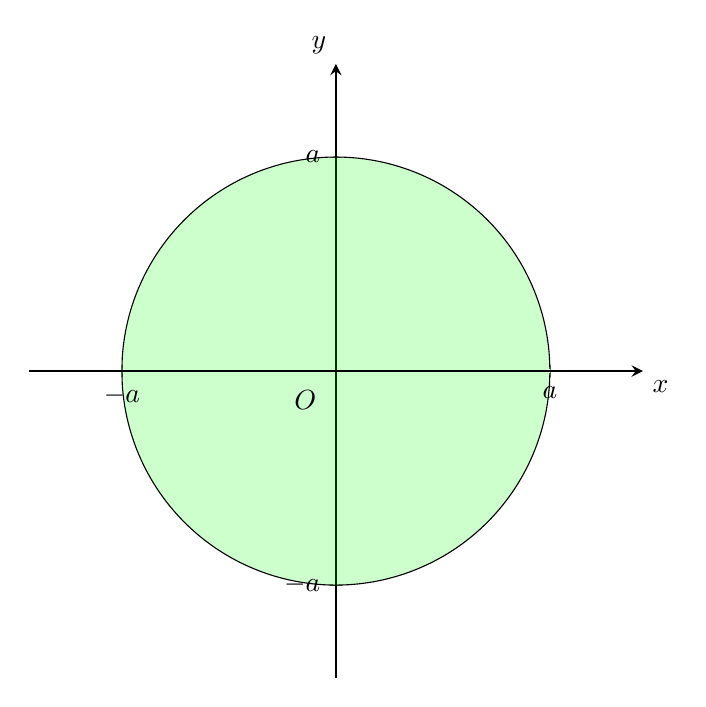
\begin{tikzpicture}
    \begin{axis}[standard,
            xtick={-2.718,2.718},
            ytick={-2.718,2.718},
            samples=1000,
            xlabel={$x$},
            ylabel={$y$},
            xmin=-3,xmax=3,
            ymin=-3,ymax=3,
            x=1cm,
            y=1cm/1,
            xticklabels={$-a$,$a$},
            yticklabels={$-a$,$a$}
           ]
\node[anchor=center,label=south west:$O$] at (axis cs:0,0){};
\addplot[name path=F,domain={-2.718:2.718}]{sqrt(2.718^2-x^2};
\addplot[name path=G,domain={-2.718:2.718}]{-sqrt(2.718^2-x^2};
\addplot[name path=H,domain={-2.718:2.718}]{0};
\addplot[fill=green, fill opacity=0.2] fill between [of=F and H, soft clip={domain=-2.718:2.718}];
\addplot[fill=green, fill opacity=0.2] fill between [of=G and H, soft clip={domain=-2.718:2.718}];
    \end{axis}
    \end{tikzpicture}
}
\end{center}
Our lower and upper bounds for $r$ are $r=0$ and $r=a$, respectively.

Our lower and upper bounds for $t$ are $t=0$ and $t=2\pi$, respectively.

Let's evaluate the integral.
\begin{align*}
    \oint_C \F\cdot d\r&=\int_0^{2\pi}\int_0^a \lrp{1 - (-1)} r\,dr\,d\theta\\
    &=\int_0^{2\pi} \int_0^a 2r\,dr\,d\theta\\
    &=\int_0^{2\pi} \lrb{r^2}_0^a \,d\theta\\
    &=\int_0^{2\pi} a^2 \,d\theta\\
    &=\lrb{a^2\theta}_0^{2\pi}\\
    &=\boxed{2\pi a^2}
\end{align*}

\phantomsection
\addcontentsline{toc}{subsection}{1(b)}\textbf{(b)} $\F(x,y)=\lra{-x^2y,xy}$

\Solution

\phantomsection
\addcontentsline{toc}{subsubsection}{Direct Method}\textbf{Direct Method}

Recall that the direct method for evaluating $\displaystyle \oint_C \F\cdot d\r$ is
\begin{align*}
    \int_C \F\cdot d\r&=\int_a^b \F\lrp{\r(t)}\cdot \r'(t)\,dt
\end{align*}
If $\r(t)=\lra{a\cos t, a\sin t}$, then
\begin{align*}
    \F\lrp{\r(t)}&=\lra{-\lrp{a\cos t}^2 \lrp{a\sin t}, \lrp{a\cos t}\lrp{a\sin t}^2}=\lra{-a^3\cos^2 t\sin t,a^3\cos t\sin^2t}\\
    \r'(t)&=\lra{-a\sin t,a \cos t}
\end{align*}
Let's evaluate the integral.
\begin{align*}
    \oint_C \F\cdot d\r&=\int_0^{2\pi}\lra{-a^3\cos^2 t\sin t,a^3\cos t\sin^2t}\cdot \lra{-a\sin t,a \cos t}\,dt\\
    &=\int_0^{2\pi} a^4\cos^2 t\sin^2 t + a^4 \cos^2t \sin^2t\,dt\\
    &=\int_0^{2\pi} 2a^4\cos^2 t\sin^2 t\,dt\\
    &=2a^4\int_0^{2\pi} \cos^2 t\sin^2 t\,dt\tag{we can take constants out}\\
    &=2a^4 \int_0^{2\pi}\lrp{\cos t\sin t}^2\,dt\\
    &=2a^4 \int_0^{2\pi} \lrp{\frac{1}{2}\sin 2t}^2 \,dt\tag{$\sin 2t = 2\cos t\sin t$}\\
    &=2a^4 \int_0^{2\pi} \frac{1}{4}\sin^2 2t\,dt\\
    &=2a^4 \int_0^{2\pi} \frac{1}{4}\Bigg(\frac{1}{2}\lrp{1-\cos 4t}\Bigg)\,dt\tag{$\sin^2 t = \frac{1}{2}\lrp{1-\cos 2t}$}\\
    &=2a^4\lrp{\frac{1}{4}}\lrp{\frac{1}{2}}\int_0^{2\pi}1-\cos 4t\,dt\tag{we can take constants out}\\
    &=\frac{a^4}{4}\lrb{t-\frac{1}{4}\sin 4t}_0^{2\pi}\\
    &=\frac{a^4}{4}\Bigg(\lrp{2\pi - \frac{1}{4}\sin 8\pi}-\lrp{0-\frac{1}{4}\sin 0}\Bigg)\\
    &=\frac{a^4}{4}\lrp{2\pi - 0 - 0 + 0}\\
    &=\boxed{\frac{\pi a^4}{2}}
\end{align*}
\phantomsection
\addcontentsline{toc}{subsubsection}{Green's Theorem}\textbf{Green's Theorem}

Recall that the Green's Theorem states that
\begin{align*}
    \int_C \mathbf{F} \cdot d\mathbf{r} = \iint_R \frac{\partial N}{\partial x} - \frac{\partial M}{\partial y}\,dA
\end{align*}
If $\F(x,y)=\lra{-x^2y,xy^2}$, then
\begin{align*}
    M=-x^2y&\implies \frac{\partial M}{\partial y}=-x^2\\
    N=xy^2&\implies \frac{\partial N}{\partial x}= y^2
\end{align*}
To find our region $R$, let's graph the circle $\r(t)=\lra{a\cos t, a\sin t}$, $0\leq t\leq 2\pi$.
\begin{center}
\resizebox{3.5cm}{!}{
    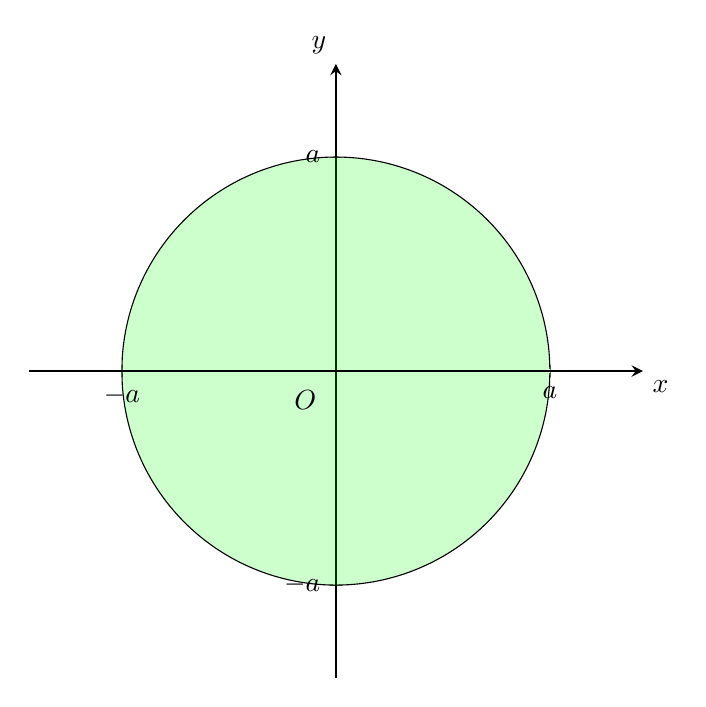
\begin{tikzpicture}
    \begin{axis}[standard,
            xtick={-2.718,2.718},
            ytick={-2.718,2.718},
            samples=1000,
            xlabel={$x$},
            ylabel={$y$},
            xmin=-3,xmax=3,
            ymin=-3,ymax=3,
            x=1cm,
            y=1cm/1,
            xticklabels={$-a$,$a$},
            yticklabels={$-a$,$a$}
           ]
\node[anchor=center,label=south west:$O$] at (axis cs:0,0){};
\addplot[name path=F,domain={-2.718:2.718}]{sqrt(2.718^2-x^2};
\addplot[name path=G,domain={-2.718:2.718}]{-sqrt(2.718^2-x^2};
\addplot[name path=H,domain={-2.718:2.718}]{0};
\addplot[fill=green, fill opacity=0.2] fill between [of=F and H, soft clip={domain=-2.718:2.718}];
\addplot[fill=green, fill opacity=0.2] fill between [of=G and H, soft clip={domain=-2.718:2.718}];
    \end{axis}
    \end{tikzpicture}
}
\end{center}
Our lower and upper bounds for $r$ are $r=0$ and $r=a$, respectively.

Our lower and upper bounds for $t$ are $t=0$ and $t=2\pi$, respectively.

Let's evaluate the integral.
\begin{align*}
    \oint_C \F\cdot d\r&=\int_0^{2\pi}\int_0^a \lrp{r^2}r\,dr\,d\theta\\
    &=\int_0^{2\pi}\int_0^a r^3\,dr\,d\theta\\
    &=\int_0^{2\pi}\lrb{\frac{1}{4}r^4}_0^a\,d\theta\\
    &=\int_0^{2\pi} \frac{1}{4}a^4\,d\theta\\
    &=\lrb{\frac{1}{4}a^4\theta}_0^{2\pi}\\
    &=\boxed{\frac{\pi a^4}{2}}
\end{align*}
\phantomsection
\addcontentsline{toc}{section}{Problem 2 (Parts)}\textbf{Problem 2 (Parts)}

Find the circulation and flux for the vector field $\F$ around and across the curve $C$:

\phantomsection
\addcontentsline{toc}{subsection}{2(a)}\textbf{(a)} $\F(x,y)=\lra{x^2+4y,x+y^2}$, $C$ is the square bounding $0\leq x\leq 1$, $0\leq y\leq 1$

\Solution

\phantomsection
\addcontentsline{toc}{subsubsection}{Circulation}\textbf{Circulation}

Recall that circulation for a vector field $\F$ around and across a curve $C$ is
\begin{equation*}
    \text{circulation}= \iint_R \frac{\partial N}{\partial x} - \frac{\partial M}{\partial y}\,dA
\end{equation*}
If $\F(x,y)=\lra{x^2+4y,x+y^2}$, $C$, then
\begin{align*}
    M=x^2+4y &\implies \frac{\partial M}{\partial y}=4\\
    N=x+y^2&\implies \frac{\partial N}{\partial x}=1
\end{align*}
As stated in the problem, the lower and upper bounds of $y$ are $y=0$ and $y=1$, respectively. 

The lower and upper bounds of $x$ are $x=0$ and $x=1$, respectively. 

Order does not matter, but I will go with $dy\,dx$ because $y$-not hahaha...

Let's evaluate the integral
\begin{align*}
    \text{circulation}&=\int_0^1\int_0^1 1 - 4\,dy\,dx\\
    &=\int_0^1 \int_0^1 -3\,dy\,dx\\
    &=\int_0^1 \lrb{-3y}_0^1\,dx\\
    &=\int_0^1 -3\,dx\\
    &=\lrb{-3x}_0^1\\
    &=-3
\end{align*}
\newpage
\phantomsection
\addcontentsline{toc}{subsubsection}{Flux}\textbf{Flux}

Recall that flux for a vector field around and across a curve $C$ is
\begin{equation*}
   \text{flux} = \iint_R \frac{\partial M}{\partial x} + \frac{\partial N}{\partial y}\,dA
\end{equation*}
If $\F(x,y)=\lra{x^2+4y,x+y^2}$, $C$, then
\begin{align*}
    M=x^2+4y &\implies \frac{\partial M}{\partial x}=2x\\
    N=x+y^2&\implies \frac{\partial N}{\partial y}=2y
\end{align*}
Our region $R$ for flux is going to be the same as our region $R$ for circulation. Therefore, the flux bounds for $x$ and $y$ are the same as the circulation bounds for $x$ and $y$.

Let's evaluate the integral
\begin{align*}
    \text{flux}&=\int_0^1 \int_0^1 2x+2y\,dy\,dx\\
    &=\int_0^1 \lrb{2xy+y^2}_0^1\,dx\\
    &=\int_0^1 2x+1\,dx\\
    &=\lrb{x^2+x}_0^1\\
    &=2
\end{align*}
Our final answer is
\begin{subequations}
    \begin{empheq}[box=\widefbox]{align}
        \text{circulation}&=-3\nonumber\\
           \text{flux}&= 2 \nonumber
    \end{empheq}
\end{subequations}
\phantomsection
\addcontentsline{toc}{subsection}{2(b)}\textbf{(b)} $\F(x,y)=\lra{x+y,-x^2-y^2}$, $C$ is the triangle $y=0$, $x=1$, and $y=x$.

\Solution

\phantomsection
\addcontentsline{toc}{subsubsection}{Circulation}\textbf{Circulation}

Recall that circulation for a vector field $\F$ around and across a curve $C$ is
\begin{equation*}
    \text{circulation}= \iint_R \frac{\partial N}{\partial x} - \frac{\partial M}{\partial y}\,dA
\end{equation*}
If $\F(x,y)=\lra{x+y-x^2-y^2}$, then
\begin{align*}
    M=x+y&\implies \frac{\partial M}{\partial y}=1\\
    N=-x^2-y^2&\implies \frac{\partial N}{\partial x}=-2x
\end{align*}

To find our region $R$, let's graph the triangle $y=0$, $x=1$, and $y=x$.
\begin{center}
\resizebox{3.5cm}{!}{
    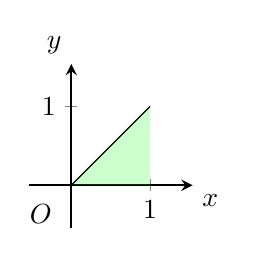
\begin{tikzpicture}
    \begin{axis}[standard,
            xtick={1},
            ytick={1},
            samples=1000,
            xlabel={$x$},
            ylabel={$y$},
            xmin=-0.3,xmax=1.3,
            ymin=-.3,ymax=1.3,
            x=1cm,
            y=1cm/1,
           ]
\node[anchor=center,label=south west:$O$] at (axis cs:0,0){};
\addplot[name path=F,domain={0:1}]{x};
\addplot[name path=G,domain={0:1}]{0};
\addplot[fill=green, fill opacity=0.2] fill between [of=F and G, soft clip={domain=0:1}];
    \end{axis}
    \end{tikzpicture}
}
\end{center}
Our lower and upper bounds for $y$ are $y=0$ and $y=x$, respectively.

Our lower and upper bounds for $x$ are $x=0$ and $x=1$, respectively.

Let's evaluate the integral
\begin{align*}
    \text{circulation}&=\int_0^1 \int_0^x -2x - 1\,dy\,dx\\
    &=\int_0^1 \lrb{-2xy-y}_0^x\,dx\\
    &=\int_0^1 -2x^2 - x\,dx\\
    &=\lrb{-\frac{2}{3}x^3-\frac{1}{2}x^2}_0^1\\
    &=-\frac{2}{3}-\frac{1}{2}\\
    &=-\frac{7}{6}
\end{align*}

\phantomsection
\addcontentsline{toc}{subsubsection}{Flux}\textbf{Flux}

Recall that flux for a vector field around and across a curve $C$ is
\begin{equation*}
   \text{flux} = \iint_R \frac{\partial M}{\partial x} + \frac{\partial N}{\partial y}\,dA
\end{equation*}
If $\F(x,y)=\lra{x+y,-x^2-y^2}$, then
\begin{align*}
    M=x+y &\implies \frac{\partial M}{\partial x}=1\\
    N=-x^2-y^2&\implies \frac{\partial N}{\partial y}=-2y
\end{align*}
Our region $R$ for flux is going to be the same as our region $R$ for circulation. Therefore, the flux bounds for $x$ and $y$ are the same as the circulation bounds for $x$ and $y$.

Let's evaluate the integral
\begin{align*}
    \text{flux}&=\int_0^1 \int_0^x 1-2y\,dy\,dx\\
    &=\int_0^1 \lrb{y-y^2}_0^x\,dx\\
    &=\int_0^1 x-x^2\,dx\\
    &=\lrp{\frac{1}{2}x-\frac{1}{3}x^3}_0^1\\
    &=\frac{1}{2}-\frac{1}{3}\\
    &=\frac{1}{6}
\end{align*}
Our final answer is
\begin{subequations}
    \begin{empheq}[box=\widefbox]{align}
        \text{circulation}&=-\frac{7}{6}\nonumber\\
           \text{flux}&= \frac{1}{6} \nonumber
    \end{empheq}
\end{subequations}
\newpage
\phantomsection
\addcontentsline{toc}{subsection}{2(c)}\textbf{(c)} $\F(x,y)=\lra{xy+y^2,x-y}$, $C$ consists of $y=x^2$ from $(0,0)$ to $(1,1)$ and $x=y^2$ from $(1,1)$ to $(0,0)$

\Solution

\phantomsection
\addcontentsline{toc}{subsubsection}{Circulation}\textbf{Circulation}

Recall that circulation for a vector field $\F$ around and across a curve $C$ is
\begin{equation*}
    \text{circulation}= \iint_R \frac{\partial N}{\partial x} - \frac{\partial M}{\partial y}\,dA
\end{equation*}
If $\F(x,y)=\lra{xy+y^2,x-y}$, then
\begin{align*}
    M=xy+y^2&\implies \frac{\partial M}{\partial y}=x+2y\\
    N=x-y&\implies \frac{\partial N}{\partial x}=1
\end{align*}

To find our region $R$, let's graph $y=x^2$ from $(0,0)$ to $(1,1)$ and $x=y^2$ from $(1,1)$ to $(0,0)$.
\begin{center}
\resizebox{3.5cm}{!}{
    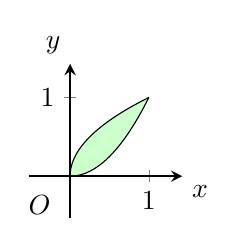
\begin{tikzpicture}
    \begin{axis}[standard,
            xtick={1},
            ytick={1},
            samples=1000,
            xlabel={$x$},
            ylabel={$y$},
            xmin=-0.3,xmax=1.2,
            ymin=-.3,ymax=1.2,
            x=1cm,
            y=1cm/1,
           ]
\node[anchor=center,label=south west:$O$] at (axis cs:0,0){};
\addplot[name path=F,domain={0:1}]{x^2};
\addplot[name path=G,domain={0:1}]{sqrt(x)};
\addplot[fill=green, fill opacity=0.2] fill between [of=F and G, soft clip={domain=0:1}];
    \end{axis}
    \end{tikzpicture}
}
\end{center}
Note that $x=y^2$ can be rewritten as $y=\pm \sqrt{x}$.

Our lower and upper bounds for $y$ are $y=x^2$ and $y=\sqrt{x}$, respectively.

Our lower and upper bounds for $x$ are $x=0$ and $x=1$, respectively.

Let's evaluate the integral.
\begin{align*}
    \text{circulation}&=\int_0^1\int_{x^2}^{\sqrt{x}}1-\lrp{x+2y}\,dy\,dx\\
    &=\int_0^1 \int_{x^2}^{\sqrt{x}}1-x-2y\,dy\,dx\\
    &=\int_0^1 \lrb{y-xy-y^2}_{x^2}^{\sqrt{x}}\,dx\\
    &=\int_0^1 \lrp{{x}^{1/2}-x^{3/2}-x}-\lrp{x^2-x^3-x^4}\,dx\\
    &=\int_0^1 x^{1/2}-x-x^{3/2}-x^2+x^3+x^4\,dx\\
    &=\lrb{\frac{2}{3}x^{3/2}-\frac{1}{2}x^2-\frac{2}{5}x^{5/2}-\frac{1}{3}x^3+\frac{1}{4}x^4+\frac{1}{5}x^5}_0^1\\
    &=\frac{2}{3}-\frac{1}{2}-\frac{2}{5}-\frac{1}{3}+\frac{1}{4}+\frac{1}{5}\\
    &=-\frac{7}{60}\tag{use a calculator}
\end{align*}
\newpage
\phantomsection
\addcontentsline{toc}{subsubsection}{Flux}\textbf{Flux}

Recall that flux for a vector field around and across a curve $C$ is
\begin{equation*}
   \text{flux} = \iint_R \frac{\partial M}{\partial x} + \frac{\partial N}{\partial y}\,dA
\end{equation*}
If $\F(x,y)=\lra{xy+y^2,x-y}$, then
\begin{align*}
    M=xy+y^2 &\implies \frac{\partial M}{\partial x}=y\\
    N=-x-y&\implies \frac{\partial N}{\partial y}=-1
\end{align*}
Our region $R$ for flux is going to be the same as our region $R$ for circulation. Therefore, the flux bounds for $x$ and $y$ are the same as the circulation bounds for $x$ and $y$.

Let's evaluate the integral.
\begin{align*}
    \text{flux}&=\int_0^1\int_{x^2}^{\sqrt{x}}y+\lrp{-1}\,dy\,dx\\
    &=\int_0^1\int_{x^2}^{\sqrt{x}}y-1\,dy\,dx\\
    &=\int_0^1 \lrb{\frac{1}{2}y^2 -y}_{x^2}^{\sqrt{x}}\,dx\\
    &=\int_0^1 \lrp{\frac{1}{2}x-x^{1/2}}-\lrp{\frac{1}{2}x^4-x^2}\,dx\\
    &=\int_0^1 \frac{1}{2}x-x^{1/2}-\frac{1}{2}x^4+x^2\,dx\\
    &=\lrb{\frac{1}{4}x^2-\frac{2}{3}x^{3/2}-\frac{1}{10}x^5+\frac{1}{3}x^3}_0^1\\
    &=\frac{1}{4}-\frac{2}{3}-\frac{1}{10}+\frac{1}{3}\\
    &=-\frac{11}{60}\tag{use a calculator}
\end{align*}
Our final answer is
\begin{subequations}
    \begin{empheq}[box=\widefbox]{align}
        \text{circulation}&=-\frac{7}{60}\nonumber\\
           \text{flux}&= -\frac{11}{60} \nonumber
    \end{empheq}
\end{subequations}

\phantomsection
\addcontentsline{toc}{subsection}{2(d)}\textbf{(d)} $\displaystyle \F(x,y)=\lra{\tan^{-1}\frac{x}{y},\ln(x^2+y^2)}$, $C$ is the curve bounding $1\leq r\leq 2$, $0\leq \theta\leq \pi$

\Solution

\phantomsection
\addcontentsline{toc}{subsubsection}{Circulation}\textbf{Circulation}

Recall that circulation for a vector field $\F$ around and across a curve $C$ is
\begin{equation*}
    \text{circulation}= \iint_R \frac{\partial N}{\partial x} - \frac{\partial M}{\partial y}\,dA
\end{equation*}
If $\displaystyle\F(x,y)=\lra{\tan^{-1}\frac{x}{y},\ln(x^2+y^2)}$, then
\begin{align*}
    M=\tan^{-1}\frac{x}{y}&\implies \frac{\partial M}{\partial y}=\frac{1}{1+\frac{x^2}{y^2}}\lrp{-\frac{x}{y^2}}=-\frac{x}{y^2+x^2}\\
    N=\ln(x^2+y^2)&\implies \frac{\partial N}{\partial x}=\frac{2x}{x^2+y^2}
\end{align*}
To find our region $R$, let's graph $1\leq r\leq 2$ from $0\leq \theta\leq \pi$.
\begin{center}
\resizebox{4cm}{!}{
    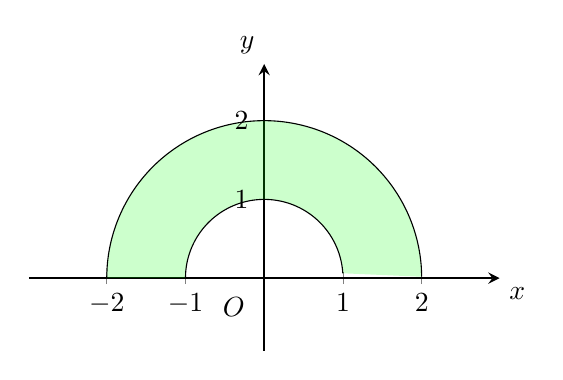
\begin{tikzpicture}
    \begin{axis}[standard,
            xtick={-2,-1,1,2},
            ytick={1,2},
            samples=1000,
            xlabel={$x$},
            ylabel={$y$},
            xmin=-2.3,xmax=2.3,
            ymin=-0.5,ymax=2.3,
            x=1cm,
            y=1cm/1,
           ]
\node[anchor=center,label=south west:$O$] at (axis cs:0,0){};
\addplot[name path=F,domain={-2:2}]{0};
\addplot[name path=G,domain={-2:2}]{sqrt(4-x^2)};
\addplot[name path=H,domain={-1:1}]{sqrt(1-x^2)};
\addplot[fill=green, fill opacity=0.2] fill between [of=H and G, soft clip={domain=-2:2}];
    \end{axis}
    \end{tikzpicture}
}
\end{center}
Our lower and upper bounds for $r$ are $r=1$ and $r=2$, respectively.

Our lower and upper bounds for $\theta$ are $\theta=0$ and $\theta=\pi$, respectively.

Let's evaluate the integral.
\begin{align*}
    \text{circulation}&=\int_0^{\pi}\int_1^2 \Bigg(\frac{2r\cos \theta}{r^2}-\lrp{-\frac{r\cos \theta}{r^2}}\Bigg)r\,dr\,d\theta\\
    &=\int_0^{\pi}\int_1^2 \lrp{\frac{3r\cos \theta}{r^2}}r\,dr\,d\theta\\
    &=\int_0^{\pi}\int_1^2 \frac{3r^2\cos \theta}{r^2}\,dr\,d\theta\\
    &=\int_0^{\pi}\int_1^2  3\cos \theta\,dr\,d\theta\\
    &=\int_0^{\pi}\lrb{3r\cos \theta }_1^2 \,d\theta\\
    &=\int_0^{\pi}6\cos \theta - 3\cos \theta\,d\theta\\
    &=\int_0^{\pi}3\cos\theta\,d\theta\\
    &=\lrb{3\sin \theta}_0^{\pi}\\
    &=3\sin \pi - 3\sin 0\\
    &= 0 - 0\\
    &=\boxed{0}
\end{align*}

\phantomsection
\addcontentsline{toc}{subsubsection}{Flux}\textbf{Flux}

Recall that flux for a vector field around and across a curve $C$ is
\begin{equation*}
   \text{flux} = \iint_R \frac{\partial M}{\partial x} + \frac{\partial N}{\partial y}\,dA
\end{equation*}
If $\displaystyle\F(x,y)=\lra{\tan^{-1}\frac{x}{y},\ln(x^2+y^2)}$, then
\begin{align*}
    M=\tan^{-1}\frac{x}{y}&\implies \frac{\partial M}{\partial x}=\frac{1}{1+\frac{x^2}{y^2}}\lrp{\frac{1}{y}}=\frac{1}{y+\frac{x^2}{y}}=\frac{y}{y^2+x^2}\\
    N=\ln(x^2+y^2)&\implies \frac{\partial N}{\partial y}=\frac{2y}{x^2+y^2}
\end{align*}
Our region $R$ for flux is going to be the same as our region $R$ for circulation. Therefore, the flux bounds for $\theta$ and $r$ are the same as the circulation bounds for $\theta$ and $r$.

Let's evaluate the integral
\begin{align*}
    \text{flux}&=\int_0^\pi\int_1^2 \lrp{\frac{r\sin \theta}{r^2}+\frac{2r\sin \theta}{r^2}}r\,dr\,d\theta\\
    &=\int_0^{\pi}\int_1^2 \lrp{\frac{3r\sin \theta}{r^2}}r\,dr\,d\theta\\
    &=\int_0^\pi \int_1^2 \frac{3r^2\sin\theta}{r^2}\,dr\,d\theta\\
    &=\int_0^\pi \int_1^2 3\sin \theta\,dr\,d\theta\\
    &=\int_0^\pi \lrb{3r\sin \theta}_1^2\,d\theta\\
    &=\int_0^\pi 6\sin \theta -\lrp{3\sin \theta}\,d\theta\\
    &=\int_0^\pi 3\sin\theta\,d\theta\\
    &=\lrb{-3\cos \theta}_0^\pi\\
    &=-3\cos \pi - \lrp{-3\cos 0}\\
    &=\lrp{3}-\lrp{-3}\\
    &=6
\end{align*}
Our final answer is
\begin{subequations}
    \begin{empheq}[box=\widefbox]{align}
        \text{circulation}&=0\nonumber\\
           \text{flux}&= 6 \nonumber
    \end{empheq}
\end{subequations}

\phantomsection
\addcontentsline{toc}{subsection}{2(e)}\textbf{(e)} $\F(x,y)=\lra{-\sin y,x\cos y}$, $C$ is the square bounding $0\leq x\leq \dfrac{\pi}{2}$, $0\leq y\leq \dfrac{\pi}{2}$

\Solution

\phantomsection
\addcontentsline{toc}{subsubsection}{Circulation}\textbf{Circulation}

Recall that circulation for a vector field $\F$ around and across a curve $C$ is
\begin{equation*}
    \text{circulation}= \iint_R \frac{\partial N}{\partial x} - \frac{\partial M}{\partial y}\,dA
\end{equation*}
If $\F(x,y)=\lra{-\sin y,x\cos y}$, then
\begin{align*}
    M=-\sin y&\implies \frac{\partial M}{\partial y}=-\cos y\\
    N=x\cos y&\implies \frac{\partial N}{\partial x}=\cos y
\end{align*}

To find our region $R$, let's graph the square bounding $\displaystyle 0\leq x\leq \frac{\pi}{2}$, $\displaystyle 0\leq y\leq \frac{\pi}{2}$.
\begin{center}
\resizebox{3.5cm}{!}{
    \begin{tikzpicture}
    \begin{axis}[standard,
            xtick={2},
            ytick={2},
            samples=1000,
            xlabel={$x$},
            ylabel={$y$},
            xmin=-0.3,xmax=2.3,
            ymin=-.3,ymax=2.3,
            x=1cm,
            y=1cm/1,
            xticklabels={$\dfrac{\pi}{2}$},
            yticklabels={$\dfrac{\pi}{2}$}
           ]
\node[anchor=center,label=south west:$O$] at (axis cs:0,0){};
\addplot[name path=F,domain={0:2}]{0};
\addplot[name path=G,domain={0:2}]{2};
\addplot[fill=green, fill opacity=0.2] fill between [of=F and G, soft clip={domain=0:2}];
    \end{axis}
    \end{tikzpicture}
}
\end{center}
Our lower and upper bounds for $y$ are $y=0$ and $y=\dfrac{\pi}{2}$, respectively.

Our lower and upper bounds for $x$ are $x=0$ and $x=\dfrac{\pi}{2}$, respectively.

Let's evaluate the integral
\begin{align*}
    \text{circulation}&=\int_0^{\pi/2}\int_0^{\pi/2} \cos y -\lrp{-\cos y}\,dy\,dx\\
    &=\int_0^{\pi/2}\int_0^{\pi/2} 2\cos y\,dy\,dx\\
    &=\int_0^{\pi/2}\lrb{2\sin y}_0^{\pi/2}\,dx\\
    &=\int_0^{\pi/2}2\sin \frac{\pi}{2}-2\sin 0\,dx\\
    &=\int_0^{\pi/2}2\,dx\\
    &=\lrb{2x}_0^{\pi/2}\\
        &=\boxed{\pi}
\end{align*}


\phantomsection
\addcontentsline{toc}{subsubsection}{Flux}\textbf{Flux}

Recall that flux for a vector field around and across a curve $C$ is
\begin{equation*}
   \text{flux} = \iint_R \frac{\partial M}{\partial x} + \frac{\partial N}{\partial y}\,dA
\end{equation*}
If $\F(x,y)=\lra{-\sin y,x\cos y}$, then
\begin{align*}
    M=-\sin y&\implies \frac{\partial M}{\partial x}=0\\
    N=x\cos y&\implies \frac{\partial N}{\partial y}=-x\sin y
\end{align*}
Our region $R$ for flux is going to be the same as our region $R$ for circulation. Therefore, the flux bounds for $x$ and $y$ are the same as the circulation bounds for $x$ and $y$.

Let's evaluate the integral
\begin{align*}
    \text{flux}&=\int_0^{\pi/2}\int_0^{\pi/2}0 + \lrp{-x\sin y}\,dy\,dx\\
    &=\int_0^{\pi/2}\int_0^{\pi/2} -x\sin y\,dy\,dx\\
    &=\int_0^{\pi/2}\lrb{x\cos y}_0^{\pi/2}\,dx\\
    &=\int_0^{\pi/2} x\cos \frac{\pi}{2}-x\cos 0\,dx\\
    &=\int_0^{\pi/2} -x\,dx\\
    &=\lrb{-\frac{1}{2}x^2}_0^{\pi/2}\\
    &=-\frac{1}{2}\lrp{\frac{\pi}{2}}^2\\
    &=\boxed{-\frac{1}{8}\pi^2}
\end{align*}
Our final answer is
\begin{subequations}
    \begin{empheq}[box=\widefbox]{align}
        \text{circulation}&=\pi\nonumber\\
           \text{flux}&= -\frac{1}{8}\pi^2\nonumber
    \end{empheq}
\end{subequations}

\phantomsection
\addcontentsline{toc}{subsection}{2(f)}\textbf{(f)} $\displaystyle \F(x,y)=\lra{\frac{x}{1+y^2},\tan^{-1}y}$, $C$ is the circle $x^2+y^2=1$

\Solution

\phantomsection
\addcontentsline{toc}{subsubsection}{Circulation}\textbf{Circulation}

Recall that circulation for a vector field $\F$ around and across a curve $C$ is
\begin{equation*}
    \text{circulation}= \iint_R \frac{\partial N}{\partial x} - \frac{\partial M}{\partial y}\,dA
\end{equation*}
If $\displaystyle\F(x,y)=\lra{\frac{x}{1+y^2},\tan^{-1}y}$, then
\begin{align*}
    M=\frac{x}{1+y^2}&\implies \frac{\partial M}{\partial y}=-\frac{x}{(1+y^2)^2}(2y)=-\frac{2xy}{(1+y^2)^2}\\
    N=\tan^{-1}y&\implies \frac{\partial N}{\partial x}=0
\end{align*}

To find our region $R$, let's graph the circle $x^2+y^2=1$.
\begin{center}
\resizebox{3.5cm}{!}{
    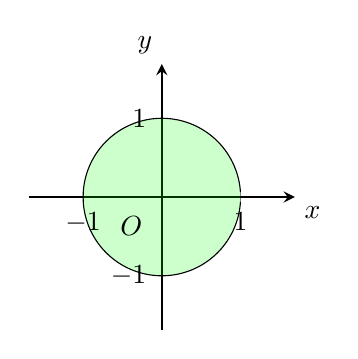
\begin{tikzpicture}
    \begin{axis}[standard,
            xtick={-1,1},
            ytick={-1,1},
            samples=1000,
            xlabel={$x$},
            ylabel={$y$},
            xmin=-1.3,xmax=1.3,
            ymin=-1.3,ymax=1.3,
            x=1cm,
            y=1cm/1
           ]
\node[anchor=center,label=south west:$O$] at (axis cs:0,0){};
\addplot[name path=F,domain={-1:1}]{sqrt(1-x^2};
\addplot[name path=G,domain={-1:1}]{-sqrt(1-x^2};
\addplot[fill=green, fill opacity=0.2] fill between [of=F and G, soft clip={domain=-1:1}];
    \end{axis}
    \end{tikzpicture}
}
\end{center}
Our lower and upper bounds for $y$ are $y=-\sqrt{1-x^2}$ and $y=\sqrt{1-x^2}$, respectively.

Our lower and upper bounds for $x$ are $x=-1$ and $x=1$, respectively.

Let's evaluate our integral
\begin{align*}
    \text{circulation}&=\int_{-1}^{1}\int_{-\sqrt{1-x^2}}^{\sqrt{1-x^2}} 0-\lrp{-\frac{2xy}{(1+y^2)^2}}\,dy\,dx\\
    &=\int_{-1}^{1}\int_{-\sqrt{1-x^2}}^{\sqrt{1-x^2}}\frac{2xy}{(1+y^2)^2}\,dy\,dx\\
    &u=1+y^2\hspace{2em}du=2y\,dy\\
    &u\lrp{-\sqrt{1-x^2}}=1+\lrp{-\sqrt{1-x^2}}^2=1+\lrp{1-x^2}=2-x^2\\
    &u\lrp{\sqrt{1-x^2}}=1+\lrp{\sqrt{1-x^2}}^2=1+\lrp{1-x^2}=2-x^2\\
    &=\int_{-1}^1 \int_{2-x^2}^{2-x^2}\frac{x}{u^2}\,du\,dx\\
    &=\int_{-1}^1 0\,dx\tag{same upper and lower bounds}\\
    &=0
\end{align*}

\newpage
\phantomsection
\addcontentsline{toc}{subsubsection}{Flux}\textbf{Flux}

Recall that flux for a vector field around and across a curve $C$ is
\begin{equation*}
   \text{flux} = \iint_R \frac{\partial M}{\partial x} + \frac{\partial N}{\partial y}\,dA
\end{equation*}
If $\displaystyle\F(x,y)=\lra{\frac{x}{1+y^2},\tan^{-1}y}$, then
\begin{align*}
    M=\frac{x}{1+y^2}&\implies \frac{\partial M}{\partial x}=\frac{1}{1+y^2}\\
    N=\tan^{-1}y&\implies \frac{\partial N}{\partial y}=\frac{1}{1+y^2}
\end{align*}
Our region $R$ for flux is going to be the same as our region $R$ for circulation. Therefore, the flux bounds for $x$ and $y$ are the same as the circulation bounds for $x$ and $y$.

Let's evaluate our integral
\begin{align*}
    \text{flux}&=\int_{-1}^1\int_{-\sqrt{1-x^2}}^{\sqrt{1-x^2}}\frac{1}{1+y^2}+\frac{1}{1+y^2}\,dy\,dx\\
    &=\int_{-1}^1\int_{-\sqrt{1-x^2}}^{\sqrt{1-x^2}}\frac{2}{1+y^2}\,dy\,dx\\
\end{align*}
You know... this integral looks like a good candidate for polar. 

Let's graph the region $y=\pm\sqrt{1-x^2}$ from $x=-1$ to $x=1$ to figure out what our region would look like in polar.
\begin{center}
\resizebox{3.5cm}{!}{
    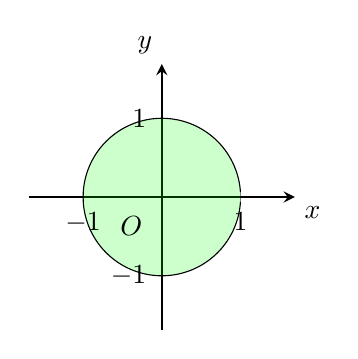
\begin{tikzpicture}
    \begin{axis}[standard,
            xtick={-1,1},
            ytick={-1,1},
            samples=1000,
            xlabel={$x$},
            ylabel={$y$},
            xmin=-1.3,xmax=1.3,
            ymin=-1.3,ymax=1.3,
            x=1cm,
            y=1cm/1,
           ]
\node[anchor=center,label=south west:$O$] at (axis cs:0,0){};
\addplot[name path=F,domain={-1:1}]{sqrt(1-x^2)};
\addplot[name path=G,domain={-1:1}]{-sqrt(1-x^2};
\addplot[fill=green, fill opacity=0.2] fill between [of=F and G, soft clip={domain=-1:1}];
    \end{axis}
    \end{tikzpicture}
}
\end{center}
Our lower and upper bounds for $r$ are $r=0$ and $r=1$, respectively.

Our lower and upper bounds for $\theta$ are $\theta=0$ and $\theta=2\pi$, respectively.

Don't forget we need to change our integrand into polar, and multiply by $r$!

Recall that in polar, $y=r\sin \theta$. Therefore,
\begin{align*}
    \frac{2}{1+y^2}=\frac{2}{1+r^2\sin^2\theta}
\end{align*}
Let's keep evaluating the integral.
\begin{align*}
    \text{flux}&=\int_{-1}^1\int_{-\sqrt{1-x^2}}^{\sqrt{1-x^2}}\frac{2}{1+y^2}\,dy\,dx\\
    &=\int_0^{2\pi}\int_0^1 \lrp{\frac{2}{1+r^2\sin^2\theta}}r\,dr\,d\theta\\
    &=\int_0^{2\pi}\int_0^1 \frac{2r}{1+r^2\sin^2\theta}\,dr\,d\theta\\
    &u=r^2\sin^2\theta\hspace{2em}du=2r\sin^2\theta\,dr\\
    &u(0)=0\hspace{2em}u(1)=\sin^2\theta\\
    &=\int_0^{2\pi}\int_0^{\sin^2\theta}\lrp{\frac{1}{1+u}}\frac{1}{\sin^2\theta}\,du\,d\theta\\
    &=\int_0^{2\pi}\lrb{\ln \left|1+u\right|\frac{1}{\sin^2\theta}}_0^{\sin^2\theta}\,d\theta\tag{$\theta$ is just a constant}\\
    &=\int_0^{2\pi}\frac{\ln (1+\sin^2\theta)}{\sin^2\theta}-\frac{\ln (1+0)}{\sin^2\theta}\,d\theta\tag{ok to drop abs since $\sin^2 \theta\geq0$}\\
    &=\int_0^{2\pi}\frac{\ln(1+\sin^2\theta)}{\sin^2\theta}\,d\theta\tag{$\ln(1)=0$}
\end{align*}
Let's make sure our region makes sense before we go any further.

Below is a graph of $\displaystyle y=\frac{\ln (1+\sin^2 \theta)}{\sin^2 \theta}$ from $\theta=0$ to $\theta=2\pi$.
\begin{center}
\resizebox{6cm}{!}{
    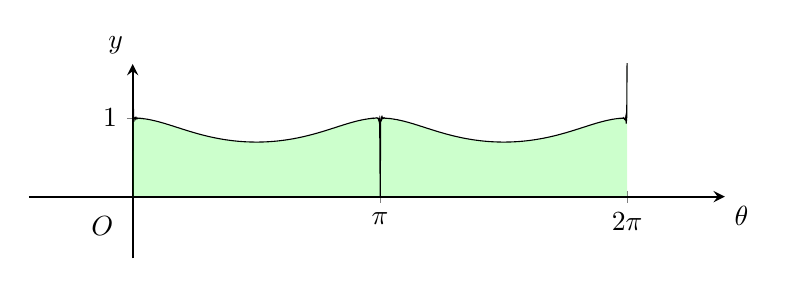
\begin{tikzpicture}
    \begin{axis}[standard,
            xtick={3.14,6.28},
            ytick={1},
            samples=1000,
            xlabel={$\theta$},
            ylabel={$y$},
            xmin=-0.3,xmax=6.5,
            ymin=-.5,ymax=1.4,
            x=1cm,
            y=1cm/1, xticklabels={$\pi$,$2\pi$}
           ]
\node[anchor=center,label=south west:$O$] at (axis cs:0,0){};
\addplot[name path=F,domain={0:6.28}]{0};
\addplot[name path=G,domain={0:6.28}]{ln(1+(sin x)^2)/(sin x)^2};
\addplot[fill=green, fill opacity=0.2] fill between [of=F and G, soft clip={domain=0:6.28}];
    \end{axis}
    \end{tikzpicture}
}
\end{center}
You'll notice that the graph from $\theta=0$ to $\theta=2\pi$ looks similar to the portion of the graph from $\theta=0$ to $\theta=\dfrac{\pi}{2}$. If we just evaluate the integral from $\theta=0$ to $\theta=2\pi$, we will be ignoring a lot of things and end up with an answer that makes no sense (use a calculator to check). Let's just evaluate the integral from $\theta=0$ to $\theta=\dfrac{\pi}{2}$ and multiply that integral by $4$ to get the whole area from $\theta=0$ to $\theta=2\pi$.

Let's keep evaluating the integral.
\begin{align*}
    \text{flux}&=\int_0^{2\pi}\frac{\ln(1+\sin^2\theta)}{\sin^2\theta}\,d\theta\\
    &=4\int_0^{\pi/2}\frac{\ln(1+\sin^2\theta)}{\sin^2\theta}\,d\theta
\end{align*}
Ok. Things are going to get a lot more hairy from here. Trust me when I say we want to multiple the integral by $4$ and evaluate the bounds ($0$ and $\pi/2$) at the end.

Let's just find what $\displaystyle \int \frac{\ln (1+\sin^2\theta)}{\sin^2\theta}\,d\theta$ is.

Using integration by parts,
\begin{align*}
   \int \frac{\ln (1+\sin^2\theta)}{\sin^2\theta}\,d\theta&\\
   &a=\ln(1+\sin^2\theta)\hspace{2em}db=\frac{1}{\sin^2\theta}\,d\theta=\csc^2\theta\,d\theta\\
   &da=\frac{2\sin\theta\cos\theta}{1+\sin^2\theta}\,d\theta\hspace{2em}b=-\cot\theta\\
   &=-\cot \theta \ln (1+\sin^2\theta)+\int\lrp{\cot \theta}\lrp{\frac{2\sin\theta \cos\theta}{1+\sin^2\theta}}\,d\theta\\
   &=-\cot \theta \ln (1+\sin^2\theta)+\int\frac{2\cos^2\theta}{1+\sin^2\theta}\,d\theta\tag{$\cot\theta=\dfrac{\cos \theta}{\sin \theta}$}\\
    &=-\cot \theta \ln (1+\sin^2\theta)+\int\frac{2\sec^2\theta}{\sec^4\theta +\sec^2\theta\tan^2\theta}\,d\theta\tag{multiply num and den by $\sec^4\theta$}\\
    &=-\cot \theta \ln (1+\sin^2\theta)+\int\frac{2\sec^2\theta}{\lrp{\tan^2\theta+1)^2+\lrp{\lrp{\tan^2\theta+1}\tan^2\theta}}}\,d\theta\tag{$\sec^2\theta=\tan^2\theta+1$}\\
    &=-\cot \theta \ln (1+\sin^2\theta)+\int\frac{2\sec^2\theta}{\tan^4\theta+2\tan^2\theta+1+\tan^4\theta+\tan^2\theta}\,d\theta\\
    &=-\cot \theta \ln (1+\sin^2\theta)+\int\frac{2\sec^2\theta}{2\tan^4\theta + 3\tan^2\theta+1}\,d\theta\\
    &t=\tan \theta\hspace{2em}dt=\sec^2\theta\,d\theta\\
    &=-\cot \theta \ln (1+\sin^2\theta)+\int\frac{2}{2t^4+3t^2+1}\,dt\\
    &=-\cot \theta \ln (1+\sin^2\theta)+\int\frac{2}{(2t^2+1)(t^2+1)}\,dt\tag{factor}\\
    &=-\cot \theta \ln (1+\sin^2\theta)+2\int\frac{1}{(2t^2+1)(t^2+1)}\,dt
\end{align*}
We love partial fraction :)
\begin{align*}
    \frac{1}{(2t^2+1)(t^2+1)}&=\frac{At+B}{2t^2+1}+\frac{Ct+D}{t^2+1}\\
    1&=(At+B)(t^2+1)+(Ct+D)(2t^2+1)\tag{multiply both sides by $(2t^2+1)(t^2+1)$}\\
    &=At^3+At+Bt^2+B+2Ct^3+Ct+2Dt^2+D\\
    &=At^3+2Ct^3+Bt^2+2Dt^2+At+Ct+B+D\\
    &=(A+2C)t^3+(B+2D)t^2+(A+C)t+(B+D)\tag{factor}
\end{align*}
Our system of equations is
\begin{align*}
    A+2C&=0\implies A=-2C\\
    B+2D&=0\implies B=-2D\\
    A+C&=0\implies A=-C\\
    B+D&=1\implies B=1-D
\end{align*}
If $A=-2C=-C$ and $B=-2D=1-D$, then
\begin{align*}
    -2C&=-C\implies C=0\implies A=0\\
    -2D&=1-D\implies D=-1\implies B=1-(-1)=2
\end{align*}
Therefore,
\begin{align*}
    A&=0\\
    B&=2\\
    C&=0\\
    D&=-1
\end{align*}
Ok. Back to evaluating the integral...
\begin{align*}
    \int\frac{\ln(1+\sin^2\theta)}{\sin^2\theta}\,d\theta&=-\cot \theta \ln (1+\sin^2\theta)+2\int\frac{0t+2}{2t^2+1}+\frac{0t+(-1)}{t^2+1}\,dt\\
    &=-\cot \theta \ln (1+\sin^2\theta)+2\int\frac{2}{2t^2+2}+\frac{-1}{t^2+1}\,dt\\
    &=-\cot \theta \ln (1+\sin^2\theta)+2\lrp{\int\frac{2}{2t^2+1}\,dt-\int\frac{1}{t^2+1}\,dt}\\
    &=-\cot \theta \ln (1+\sin^2\theta)+2\lrp{\sqrt{2}\int\frac{\sqrt{2}}{(\sqrt{2}t)^2+1}\,dt-\int\frac{1}{t^2+1}\,dt}\\
    &=-\cot \theta \ln (1+\sin^2\theta)+2\lrp{\sqrt{2}\tan^{-1}\sqrt{2}t-\tan^{-1}t}\tag{let $C=0$ aka ignore $C$}\\
    &=-\cot \theta \ln (1+\sin^2\theta)+2\sqrt{2}\tan^{-1}\sqrt{2}t-2\tan^{-1}t
\end{align*}
Since we said $t=\tan\theta$,
\begin{align*}
    \int\frac{\ln (1+\sin^2\theta)}{\sin^2\theta}\,d\theta&=-\cot \theta \ln (1+\sin^2\theta)+2\sqrt{2}\tan^{-1}t-2\tan^{-1}t\\
    &=-\cot \theta \ln (1+\sin^2\theta)+2\sqrt{2}\tan^{-1}\lrp{\sqrt{2}\tan \theta}-2\tan^{-1}\lrp{\tan\theta}\\
    &=-\cot \theta \ln (1+\sin^2\theta)+2\sqrt{2}\tan^{-1}\lrp{\sqrt{2}\tan\theta}-2\theta\tag{$\tan^{-1}$ and $\tan$ ``cancel"}
\end{align*}
Therefore,
\begin{align*}
    \int\frac{\ln (1+\sin^2\theta)}{\sin^2\theta}\,d\theta&=-\cot \theta \ln (1+\sin^2\theta)+2\sqrt{2}\tan^{-1}\lrp{\sqrt{2}\tan\theta}-2\theta\tag{we're ignoring $+C$}
\end{align*}
Ok now let's evaluate the bounds $\theta=0$ to $\theta=\pi/2$ and multiple the integral by $4$ to get our entire area.
\begin{align*}
    \text{flux}&=4\int_0^{\pi/2}\frac{\ln(1+\sin^2\theta)}{\sin^2\theta}\,d\theta\\
    &=4\lrb{-\cot \theta \ln (1+\sin^2\theta)+2\sqrt{2}\tan^{-1}\lrp{\sqrt{2}\tan\theta}-2\theta}_0^{\pi/2}\\
    &=4\Bigg(\lrp{-\cot\frac{\pi}{2}\ln\lrp{1+\sin^2\frac{\pi}{2}}+\lim_{b\to\frac{\pi}{2}^{-}}2\sqrt{2}\tan^{-1}\lrp{\sqrt{2}\tan b}-2\lrp{\frac{\pi}{2}}}\\
    &\hspace{4em}-\lrp{\lim_{a\to0^{+}}-\cot a\ln(1+\sin^2 a)+2\sqrt{2}\tan^{-1}\lrp{\sqrt{2}\tan 0}-2(0)}\Bigg)\\
    &=4\Bigg(\lrp{0+\lim_{b\to\frac{\pi}{2}^{-}}2\sqrt{2}\tan^{-1}\lrp{\sqrt{2}\tan b}-\pi}-\lrp{\lim_{a\to0^{+}}-\cot a\ln(1+\sin^2 a)+0-0}\Bigg)\tag{$\cos\frac{\pi}{2}=\tan0=0$}\\
    &=4\Bigg(\Big(2\sqrt{2}\tan^{-1}\lrp{\lim_{b\to\frac{\pi}{2}^{-}}\sqrt{2}\tan b}-\pi\Big)-\Big(\lim_{a\to 0^{+}}-\cot a\ln (1+\sin^2 a)\Big)\Bigg)\\
    &=4\Bigg(\lrp{2\sqrt{2}\lrp{\frac{\pi}{2}}-\pi}-\lrp{\lim_{a\to0^+}\frac{\cos a\ln(1+\sin^2 a)}{\sin a}}\Bigg)\\
    &=4\lrp{\pi\sqrt{2}-\pi}-4\lrp{\lim_{a\to 0^+}\cos a\lim_{a\to 0^+}\frac{\ln(1+\sin^2 a)}{\sin a}}\tag{limit property}\\
    &=4\lrp{\pi\sqrt{2}-\pi}-4\lrp{\lim_{a\to 0^+}\frac{\ln(1+\sin^2 a)}{\sin a}}\tag{$\cos 0=1$}\\
    &=4\lrp{\pi\sqrt{2}-\pi}-4\lrp{\lim_{u\to 0^+}\frac{\ln(1+u^2)}{u}}\tag{let $u=\sin a$, $a\to 0^+\implies u\to 0^+$}\\
    &\overset{L.H.}{=}4\lrp{\pi\sqrt{2}-\pi}-4\lrp{\lim_{u\to 0^+}\frac{\frac{2u}{1+u^2}}{1}}\\
    &=4\lrp{\pi\sqrt{2}-\pi}-4\lrp{\lim_{u\to 0^+}\frac{2u}{1+u^2}}\\
    &=4\lrp{\pi\sqrt{2}-\pi}-4\lrp{\frac{0}{1+0^2}}\\
    &=4\lrp{\pi\sqrt{2}-\pi}-4(0)\\
    &=4\lrp{\pi\sqrt{2}-\pi}
\end{align*}
Our final answer is
\begin{subequations}
    \begin{empheq}[box=\widefbox]{align}
        \text{circulation}&=0\nonumber\\
           \text{flux}&= 4\lrp{\pi\sqrt{2}-\pi}\nonumber
    \end{empheq}
\end{subequations}
\newpage
\phantomsection
\addcontentsline{toc}{section}{Problem 3}\textbf{Problem 3}

Evaluate $\displaystyle \int_C \F\cdot d\r$, where $\F(x,y)=\lra{2xy^3,4x^2y^2}$ and $C$ is the ``triangle" consisting of the $x$-axis, the line $x=1$, and the curve $y=x^3$, traveled counterclockwise.

\Solution

Let's use our good old pal the Green's Theorem.

Recall that the Green's Theorem states that
\begin{align*}
    \int_C \mathbf{F} \cdot d\mathbf{r} = \iint_R \frac{\partial N}{\partial x} - \frac{\partial M}{\partial y}\,dA
\end{align*}
If $\F(x,y)=\lra{2xy^3,4x^2y^2}$, then
\begin{align*}
    M=2xy^3&\implies \frac{\partial M}{\partial y}= 6xy^2\\
    N=4x^2y^2&\implies \frac{\partial N}{\partial x}=8xy^2
\end{align*}
To find our region $R$, let's graph  the ``triangle" consisting of the $x$-axis, the line $x=1$, and the curve $y=x^3$.
\begin{center}
\resizebox{3.5cm}{!}{
    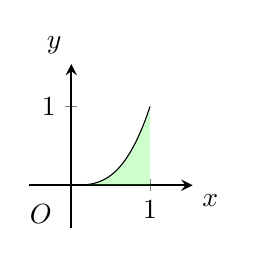
\begin{tikzpicture}
    \begin{axis}[standard,
            xtick={1},
            ytick={1},
            samples=1000,
            xlabel={$x$},
            ylabel={$y$},
            xmin=-.3,xmax=1.3,
            ymin=-.3,ymax=1.3,
            x=1cm,
            y=1cm/1
           ]
\node[anchor=center,label=south west:$O$] at (axis cs:0,0){};
\addplot[name path=F,domain={0:1}]{0};
\addplot[name path=G,domain={0:1}]{x^3};
\addplot[fill=green, fill opacity=0.2] fill between [of=F and G, soft clip={domain=0:1}];
    \end{axis}
    \end{tikzpicture}
}
\end{center}
Our lower and upper bounds for $y$ are $y=0$ and $y=x^3$, respectively.

Our lower and upper bounds for $x$ are $x=0$ and $x=1$, respectively.

Let's evaluate the integral.
\begin{align*}
    \int_C \F\cdot d\r&=\int_0^1\int_0^{x^3}8xy^2-6xy^2\,dy\,dx\\
    &=\int_0^1 \int_0^{x^3}2xy^2\,dy\,dx\\
    &=\int_0^1\lrb{\frac{2}{3}xy^3}_0^{x^3}\,dx\\
    &=\int_0^1 \frac{2}{3}x(x^3)^3\,dx\\
    &=\int_0^1 \frac{2}{3}x^{10}\,dx\tag{$x(x^3)^3=x(x^9)=x^10$}\\
    &=\lrb{\frac{2}{33}x^{11}}_0^1\\
    &=\boxed{\frac{2}{33}}
\end{align*}
\newpage
\phantomsection
\addcontentsline{toc}{section}{Problem 4 (Parts)}\textbf{Problem 4 (Parts)}

If $R$ is a plane region whose boundary curve $C$ satisfies the hypotheses of Green's Theorem, we can calculate the area of $R$ as $\displaystyle A(R)=\frac{1}{2}\oint_C x\,dy-y\,dx$.

\phantomsection
\addcontentsline{toc}{subsection}{4(a)}\textbf{(a)} Prove this statement by writing the area of R as a double integral and then using
Green’s Theorem in the reverse direction.

\Solution

Let's write the area of $R$ as a double integral. Our integrated is just going to be $1$.
\begin{align*}
    A(R)&=\iint_R\,dy\,dx\\
    &=\iint_R \frac{1}{2}+\frac{1}{2}\,dy\,dx\tag{$\displaystyle\frac{1}{2}+\frac{1}{2}=1$}
\end{align*}
Recall that Green's Theorem in the reverse direction is
\begin{align*}
     \oint_C M\,dy - N\,dx = \iint_R \frac{\partial M}{\partial x} + \frac{\partial N}{\partial y}\,dA\tag{yes, this is like flux}
\end{align*}
If $\displaystyle M=\frac{1}{2}x$ and $\displaystyle N=\frac{1}{2}y$ then,
\begin{align*}
\frac{\partial M}{\partial x}&=\frac{1}{2}\\
\frac{\partial N}{\partial y}&=\frac{1}{2}
\end{align*}
Let's keep evaluating our area of $R$ integral.
\begin{align*}
    A(R)&=\iint_R \frac{1}{2}+\frac{1}{2}\,dy\,dx\\
    &=\oint_C \frac{1}{2}x\,dy-\frac{1}{2}y\,dx\tag{Green's Theorem}\\
    &=\oint_C \frac{1}{2}\lrp{x\,dy-y\,dx}\\
    &=\frac{1}{2}\oint_C x\,dy-y\,dx\tag{we can take out constants}
\end{align*}
\qed

\phantomsection
\addcontentsline{toc}{subsection}{4(b)}\textbf{(b)} Use this to determine the area of the ellipse $\r(t)=\lra{a\cos t,b\sin t}$ and the asteroid $\r(t)=\lra{\cos^3 t,\sin ^3 t}$ (both curves are $0\leq t\leq 2\pi)$
.

\Solution

\phantomsection
\addcontentsline{toc}{subsubsection}{Ellipse} \textbf{Ellipse}

If $\r(t)=\lra{a\cos t,b\sin t}$, then
\begin{align*}
    x=a\cos t&\implies dx=-a\sin t\,dt\\
    y=b\sin t&\implies dy =b\cos t\,dt
\end{align*}
Let's evaluate our integral.
\begin{align*}
    A(R)&=\frac{1}{2}\int_0^{2\pi} \lrp{a\cos t}\lrp{b\cos t}-\lrp{b\sin t}\lrp{-a\sin t}\,dt\tag{$0\leq t\leq 2\pi$ given}\\
    &=\frac{1}{2}\int_0^{2\pi} ab\cos^2t + ab\sin^2 t\,dt\\
    &=\frac{1}{2}\int_0^{2\pi} ab\lrp{\cos^2 t+\sin^2 t}\,dt\\
    &=\frac{1}{2}\int_0^{2\pi} ab\,dt\tag{$\cos^2 t+\sin^2 t =1$}\\
    &=\frac{1}{2}\lrb{abt}_0^{2\pi}\\
    &=\frac{1}{2}\lrp{2ab\pi}\\
    &=ab\pi
\end{align*}

\phantomsection
\addcontentsline{toc}{subsubsection}{Asteroid} \textbf{Asteroid}

If $\r(t)=\lra{\cos^3 t,\sin^3 t}$, then
\begin{align*}
    x=\cos^3 t&\implies dx = -3\cos^2 t\sin t\,dt\\
    y=\sin^3 t&\implies dy=3\sin^2 t\cos t\,dt
\end{align*}
Let's evaluate our integral.
\begin{align*}
    A(R)&=\frac{1}{2}\int_0^{2\pi}\lrp{\cos^3 t}\lrp{3\sin^2 t\cos t}-\lrp{\sin^3 t}\lrp{-3\cos ^2 t\sin t}\,dt\tag{$0\leq t\leq 2\pi$ given}\\
    &=\frac{1}{2}\int_0^{2\pi}3\sin^2 t\cos^4 t +3\sin^4 t \cos^2 t\,dt\\
    &=\frac{1}{2}\int_0^{2\pi}\lrp{3\sin^2 t\cos^2 t}\lrp{\cos^2 t+\sin^2t}\,dt\\
    &=\frac{1}{2}\int_0^{2\pi}3\sin^2 t\cos ^2t\,dt\tag{$\cos^2t+\sin^2 t=1$}\\
    &=\frac{3}{2}\int_0^{2\pi}\sin^2 t\cos^2 t\,dt\tag{we can take out constants}\\
    &=\frac{3}{2}\int_0^{2\pi}\lrp{\sin t\cos t}^2\,dt\\
    &=\frac{3}{2}\int_0^{2\pi}\lrp{\frac{1}{2}\sin 2t}^2\,dt\tag{$\sin 2t=2\sin t\cos t$}\\
    &=\frac{3}{2}\int_0^{2\pi}\frac{1}{4}\sin^2 2t\,dt\\
    &=\frac{3}{8}\int_0^{2\pi}\sin^2 2t\,dt\tag{we can take out constants}\\
    &=\frac{3}{8}\int_0^{2\pi}\frac{1}{2}\lrp{1-\cos 4t}\,dt\tag{$\sin^2 t=\frac{1}{2}\lrp{1-\cos 2t}$}\\
    &=\frac{3}{16}\int_0^{2\pi}1-\cos 4t\,dt\tag{we can take out constants}\\
    &=\frac{3}{16}\lrb{t -\frac{1}{4}\sin 4t}_0^{2\pi}\\
    &=\frac{3}{16}\Bigg(\lrp{2\pi -\frac{1}{4}\sin8\pi}-\lrp{0-\frac{1}{4}\sin 0}\Bigg)\\
    &=\frac{3}{16}\lrp{2\pi -0-0+0}\\
    &=\boxed{\frac{3\pi}{8}}
\end{align*}
Our final answer is
\begin{subequations}
    \begin{empheq}[box=\widefbox]{align}
        \text{ellipse area}&=ab\pi\nonumber\\
           \text{asteroid area}&= \frac{3\pi}{8}\nonumber
    \end{empheq}
\end{subequations}
\phantomsection
\addcontentsline{toc}{subsection}{4(c)}\textbf{(c)} Show that we can also write $\displaystyle A(R)=\oint_C x\,dy=-\oint_C y\,dx$.

\Solution

We'll use similar logic to 4(a).

\phantomsection
\addcontentsline{toc}{subsubsection}{xdy} For $\displaystyle A(R)=\oint_C x\,dy$,

Let's write the area of $R$ as a double integral. Our integrated is just going to be $1$.
\begin{align*}
    A(R)&=\iint_R \,dy\,dx\\
    &=\iint_R 1 +0\,dy\,dx\tag{$1+0=1$}
\end{align*}
Recall that Green's Theorem in the reverse direction is
\begin{align*}
     \oint_C M\,dy - N\,dx = \iint_R \frac{\partial M}{\partial x} + \frac{\partial N}{\partial y}\,dA\tag{yes, this is like flux}
\end{align*}
If $\displaystyle M=x$ and $\displaystyle N=0$ then,
\begin{align*}
\frac{\partial M}{\partial x}&=1\\
\frac{\partial N}{\partial y}&=0
\end{align*}
Let's keep evaluating our area of $R$ integral.
\begin{align*}
    A(R)&=\iint_R 1+0\,dy\,dx\\
    &=\oint_C x\,dy - 0\,dx\tag{Green's Theorem}\\
    &=\oint_C x\,dy
\end{align*}

\phantomsection
\addcontentsline{toc}{subsubsection}{ydx} For $\displaystyle A(R)=\oint_C y\,dx$,

Let's write the area of $R$ as a double integral. Our integrated is just going to be $1$.
\begin{align*}
    A(R)&=\iint_R \,dy\,dx\\
    &=\iint_R 0 +1\,dy\,dx\tag{$0+1=1$}
\end{align*}
Recall that Green's Theorem in the reverse direction is
\begin{align*}
     \oint_C M\,dy - N\,dx = \iint_R \frac{\partial M}{\partial x} + \frac{\partial N}{\partial y}\,dA\tag{yes, this is like flux}
\end{align*}
If $\displaystyle M=0$ and $\displaystyle N=y$ then,
\begin{align*}
\frac{\partial M}{\partial x}&=0\\
\frac{\partial N}{\partial y}&=1
\end{align*}
Let's keep evaluating our area of $R$ integral.
\begin{align*}
    A(R)&=\iint_R 0+1\,dy\,dx\\
    &=\oint_C 0\,dy - y\,dx\tag{Green's Theorem}\\
    &=\oint_C -y\,dy\\
    &=-\oint_C y\,dy
\end{align*}
Therefore,
\begin{equation*}
    A(R)=\oint_C x\,dy=-\oint_C y\,dx
\end{equation*}

\qed

\phantomsection
\addcontentsline{toc}{section}{Problem 5}\textbf{Problem 5}

Show that the value of $\displaystyle \oint_C xy^2\,dx+(x^2y+2x)\,dy$ around any square only depends on the area of the square and not its location in the plane.

\Solution

Based on the integral,
\begin{align*}
    M=xy^2&\implies \frac{\partial M}{\partial y}=2xy\\
    N=x^2y+2x&\implies \frac{\partial N}{\partial x}=2xy+2
\end{align*}
Let's evaluate the integral.
\begin{align*}
    \oint_C xy^2\,dx+(x^2y+2x)\,dy&=\iint_R \lrp{2xy+2}-\lrp{2xy}\,dy\,dx\\
    &=\iint_R 2\,dy\,dx\\
    &=2\iint_R \,dy\,dx\\
    &=2\text{ times square area}\tag{$\text{area}=\iint_R \,dy\,dx$}
\end{align*}
Geometrically, $\displaystyle \iint_R \,dy\,dx$ represents the area of the square region. 

Therefore, the value of $\displaystyle \oint_C xy^2\,dx+(x^2y+2x)\,dy$ is equal to $2$ times the area of the square region. The location of the region is irrelevant. Only the area of the square region is needed.

\qed
\end{document}
